\documentclass[Royal,times,sageh]{sagej}

\usepackage{moreverb,url,natbib, multirow, tabularx}
\usepackage[colorlinks,bookmarksopen,bookmarksnumbered,citecolor=red,urlcolor=red]{hyperref}




\begin{document}

\title{Fake title}

\runninghead{Cimentada}

\author{Jorge Cimentada\affilnum{1}}

\affiliation{\affilnum{1}{Laboratory of Digital and Computational Demography, Max Planck Institute
of Demographic Research}}

\corrauth{Konrad-Zuse-Str. 1. Rostock, Germany}

\email{\href{mailto:cimentada@demogr.mpg.de}{\nolinkurl{cimentada@demogr.mpg.de}}}

\begin{abstract}
The literature on achievement inequality has recently started to focus
on the dynamics of the socio-economic achievement gap in cognitive
abilities. The main findings come from research in the U.S. revealing
that the 90th/10th income achievement gap has widened 50\% in the last
30 years. This chapter aims to investigate whether there are patterns in
the evolution of the achievement gap from a comparative perspective.
Using 15 years of data in 32 countries from the Program for
International Student Assessment (PISA), I find that there is
considerable variation in the way in which the gap between the average
score of students above (and at) the 90th percentile and below (and) the
10th percentile is evolving. The prime examples come from the U.S. and
Germany closing at about 50\% and 30\% in the last 15 years while France
is widening at a similar rate. I find that curricular tracking and
vocational enrollment explain 40\% of the variance in the achievement
gap between countries and show that the relationship is conditioned by a
strong interaction. Low curricular tracking is associated with a small
achievement gap, whereas high levels of curricular tracking is
associated with wide achievement gaps. However, once tracking is coupled
with high vocational enrollment this can remedy the potential adverse
effects and reduce the gap by .6 standard deviation. I use simulations
to show that switching to less curricular tracking can help decrease a
country's SES gap by about 10\% while switching to more tracking would
increase the achievement gap by about 51\% percent.
\end{abstract}

\keywords{academic achievement, education inequality, school autonomy,
international comparison}

\maketitle

\hypertarget{the-article-header-information}{%
\section{The Article Header
Information}\label{the-article-header-information}}

YAML header:

\begin{verbatim}
output:
  rticles::sim_article:
    keep_tex: TRUE
\end{verbatim}

Configure the YAML header including the following elements:

\begin{itemize}
\item
  \texttt{title}: Title
\item
  \texttt{runninghead}: Author last names, use \emph{et al.} if there
  are three or more authors.
\item
  \texttt{author}: List of author(s) containing \texttt{name} and
  \texttt{num}
\item
  \texttt{corrauth}: Corresponding author's name and address.
\item
  \texttt{email}: Correspondence email
\item
  \texttt{abstract}: Limited to 200 words
\item
  \texttt{keywords}: Keywords for the article
\item
  \texttt{bibliography}: BibTeX \texttt{.bib} file
\item
  \texttt{bibliographystyle}: sageh or sagev
\item
  \texttt{classoption}: options of the \texttt{sagej} class
\end{itemize}

\hypertarget{remarks}{%
\subsection{Remarks}\label{remarks}}

\begin{enumerate}
\def\labelenumi{\arabic{enumi}.}
\setcounter{enumi}{1}
\item
  \texttt{bibliographystyle}
\item
  \texttt{classoption}
\item
  Keywords are separated by commas.
\end{enumerate}

\hypertarget{the-body-of-the-article}{%
\section{The Body of the Article}\label{the-body-of-the-article}}

\hypertarget{mathematics}{%
\subsection{Mathematics}\label{mathematics}}

Use mathematics in Rmarkdown as usual.

\hypertarget{figures-and-tables}{%
\subsection{Figures and Tables}\label{figures-and-tables}}

Figures are supported from R code:

\begin{verbatim}
x = rnorm(10)
y = rnorm(10)
plot(x, y)
\end{verbatim}

\begin{figure}
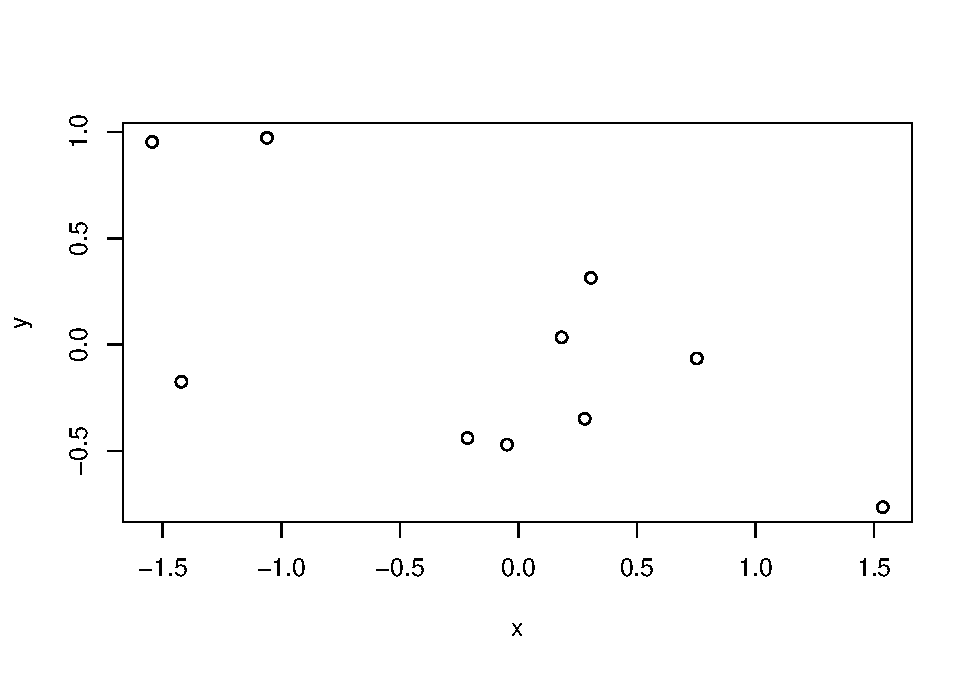
\includegraphics[width=1\linewidth]{achievement_gap_files/figure-latex/plot-ref-1} \caption{Fancy Caption\label{fig:plot}}\label{fig:plot-ref}
\end{figure}

\ldots and can be referenced (Figure \ref{fig:plot}) by including the
\texttt{\textbackslash{}\textbackslash{}label\{\}} tag in the
\texttt{fig.cap} attribute of the R chunk:
\texttt{fig.cap\ =\ "Fancy\ Caption\textbackslash{}\textbackslash{}label\{fig:plot\}"}.
It is a quirky hack at the moment, see
\href{https://github.com/yihui/knitr/issues/323}{here}.

Analogously, use Rmarkdown to produce tables as usual:

\begin{verbatim}
if (!require("xtable")) install.packages("xtable")
\end{verbatim}

\begin{verbatim}
## Loading required package: xtable
\end{verbatim}

\begin{verbatim}
xt <- xtable(head(cars), caption = "A table", label = "tab:table")
print(xt, comment = FALSE)
\end{verbatim}

\begin{table}[ht]
\centering
\begin{tabular}{rrr}
  \hline
 & speed & dist \\ 
  \hline
1 & 4.00 & 2.00 \\ 
  2 & 4.00 & 10.00 \\ 
  3 & 7.00 & 4.00 \\ 
  4 & 7.00 & 22.00 \\ 
  5 & 8.00 & 16.00 \\ 
  6 & 9.00 & 10.00 \\ 
   \hline
\end{tabular}
\caption{A table} 
\label{tab:table}
\end{table}

Referenced via \ref{tab:table}. You can also use the YAML option
\texttt{header-includes} to includes custom \LaTeX packages for tables
(keep in mind that \texttt{pandoc} uses \texttt{longtables} by default,
and it is hardcoded; some things may require including the package
\texttt{longtable}). E.g., using \texttt{ctable}:

\begin{verbatim}
header-includes:
- \usepackage{ctable}
\end{verbatim}

Then, just write straight-up \LaTeX code and reference is as usual
(\texttt{\textbackslash{}ref\{tab:ctable\}}):

\begin{verbatim}
\ctable[cap = {Short caption},
        caption = {A caption for this table.},
        label={tab:ctable},]
        {cc}
        {
        \tnote[$\ast$]{Footnote 1}
        \tnote[$\dagger$]{Other footnote}
        \tnote[b]{Mistakes are possible.}
        }{
        \FL
        COL 1\tmark[a] & COL 2\tmark[$\ast$]
        \ML
        6.92\tmark[$\dagger$] & 0.09781 \\
        6.93\tmark[$\dagger$] & 0.09901 \\
        97 & 2000
        \LL
}
\end{verbatim}

It is also possible to set the \texttt{YAML} option
\texttt{longtable:\ true} and use markdown tables (or the
\texttt{knitr::kable} function): \texttt{knitr::kable(head(cars))}
produces the same table as the \texttt{xtable} example presented before.

\hypertarget{cross-referencing}{%
\subsection{Cross-referencing}\label{cross-referencing}}

The use of the Rmarkdown equivalent of the \LaTeX cross-reference system
for figures, tables, equations, etc., is encouraged (using
\texttt{{[}@\textless{}name\textgreater{}{]}}, equivalent of
\texttt{\textbackslash{}ref\{\textless{}name\textgreater{}\}} and
\texttt{\textbackslash{}label\{\textless{}name\textgreater{}\}}). That
works well for citations in Rmarkdown, not so well for figures and
tables. In that case, it is possible to revert to standard
\LaTeX syntax.

\hypertarget{double-spacing}{%
\subsection{Double Spacing}\label{double-spacing}}

If you need to double space your document for submission please use the
\texttt{doublespace} option in the header.

\hypertarget{bibliography}{%
\section{Bibliography}\label{bibliography}}

Link a \texttt{.bib} document via the YAML header, and bibliography will
be printed at the very end (as usual). The default bibliography style is
provided by Wiley as in \texttt{WileyNJD-AMA.bst}, do not delete that
file.

Use the Rmarkdown equivalent of the \LaTeX citation system using
\texttt{{[}@\textless{}name\textgreater{}{]}}. Example:
\citep{Taylor1937}, \citep{Knupp1999, Kamm2000}.

To include all citation from the \texttt{.bib} file, add
\texttt{\textbackslash{}nocite\{*\}} before the end of the document.

\hypertarget{further-information}{%
\section{Further information}\label{further-information}}

All \LaTeX enviroments supported by the main template are supported here
as well; see the \texttt{.tex} sample file
\href{http://onlinelibrary.wiley.com/journal/10.1002/(ISSN)1097-0258/homepage/la_tex_class_file.htm}{here}
for more details and example.

\bibliographystyle{sageh}
\bibliography{bibfile}


\end{document}
